\documentclass[11pt]{article}
\usepackage{bookmark}
\usepackage{algorithm}
\usepackage{algpseudocode}
\usepackage{amsfonts}
\usepackage{amsmath}
\usepackage{amssymb}
\usepackage{amsthm}
\usepackage{bm}
\usepackage{color}
\usepackage{comment}
\usepackage{float}
\usepackage{graphicx}
%\usepackage[hidelinks]{hyperref}
\usepackage{makecell}
\usepackage[caption=false,font=footnotesize,subrefformat=parens,labelformat=parens]{subfig}
\usepackage{wrapfig}
\usepackage{url}
\usepackage[table]{xcolor}
\graphicspath{{images/}}
\setlength{\parindent}{0.25in}
\setlength{\parskip}{.05in}
\pagestyle{plain}
%Title, date an author of the document
\title{Progress Report}
\author{Bardia Mojra}


\begin{document}
\maketitle
\thispagestyle{empty}

\bigskip
\bigskip
\begin{center}
 Robotic Vision Lab
\end{center}

\begin{center}
The University of Texas at Arlington
\end{center}

\newpage

\section{Specific Research Goals}
\begin{itemize}
      \item VPQEKF (\textcolor{red}{May 30th}): Work on the paper.
      \item DLO Manipulation Dataset (ICRA - \textcolor{red}{Sept. 1st})
\end{itemize}

\section{To Do}
\begin{itemize}
  \item QEKF Paper - 30\% extension (\textcolor{red}{June 30th}):
  \begin{itemize}
      \item Read and summarize recent QEKF papers.
  \end{itemize}
  \item QEKF/QuEst+VEst Implementation (\textcolor{red}{May 30th}):
  \begin{itemize}
      \item Feature point extraction: implement semantic segmentation
      \item Address scale factor (depth-scale) issues: DL solutions?
      \item Address "hand off" issue when objects enter or leave field of view
      \item Experiments - On-going
      \item Noise issue: noise cannot be modeled - revisit
      \item Adding plots - On-going
      \item Add semantic segmentation for detecting moving object pixels and rejecting matched features in those regions
  \end{itemize}
  \item  DLO Manipulation:  \textcolor{red}{ICRA - Sept. 1st}
  \begin{itemize}
      \item Find other ICRA dataset papers and summarize the structure. --- On-going.
      \item Dynamic Dataset Collection System with Reinforcement Learning:
      \begin{itemize}
        \item Design dynamic DLO data collection system.
        \item Build work cell.
        \item Collect data and create a dataset.
        \item Define evaluation metrics.
        \item Create a high frequency RGBD dataset with UV-frames and open-loop input control actions as the ground truth.
      \end{itemize}
      \item Real-Time Preception
      \begin{itemize}
        \item Deep learning methods for keypoint pose estimation in real-time.
        \item Use UV dye dataset
        \item Use PVNet-based approach for known-objects
      \end{itemize}
      \item Learning DLO Dynamics and System Identification
      \begin{itemize}
            \item List feasible approached for learing DLO dynamics
            \item Model dynamics and deformity in a latent space
      \end{itemize}
      \item Real-Time Control
      \begin{itemize}
        \item Time model inference, using auto-encoders generate the lowest
        dimensional representation for each object.
        \item Use another GAN model for object deformity for each object.
        \item Evaluate encoded representation for accuracy.
        \item Used another GAN to explore other abstraced representations from
        individual encoded representation. In theory, we can create a low
        dimensionsal representation for multiple similar objects, given all
        individual low-dimensional representations. This is inspired by "fundamental
        principles first" approach which has universal applicability.
      \end{itemize}
  \end{itemize}
\end{itemize}


\section{Progress}
The following items are listed in the order of priority:
\begin{itemize}
    \item XEst (\textcolor{red}{RAL - April 30st, 2022}): I met with Dr. Gans
    and we went over the XEst results. I made the modules for pose and velocity
    estimations more distinct. Although the QuEst and VEst estimation methods
    are independent methods, I named pose and velocity modules QuEst+ and VEst+
    respectively. QuEst+ and VEst+ modules can contain any number of pose and
    velocity estimation modules which are the used by a corresponding QEKF filter.
    Right now, the QEKF filter instances only correspond to selected pose estimation
    methods but additional instances could be spawned for different velocity
    estimation methods on demand. This feature allows for benchmarking any
    methods and not just limited to pose and velocity estimations. Below are
    the results for QuEst+, VEst+, and QEKF modules. The entire system is called
    \emph{XEst} with \emph{X} referring modularity of the QEKF estimation system.
    Note that there are two types of error, GT-X and Z-X represent the
    groundtruth vs. the state error and the observation vs. the state, respectively.
    It is clear to me that there are some issues with computation so I am plotting
    the data logs to debug them. I need to focus on this and just wrap it up. I
    will spend this week on reading RAL EKF papers and make come up with a list
    of contributions. I am confident I can wrap this up quickly. Moreover, we
    could follow up on this paper with a double-Quaternion formulation of the
    same algorithms. It would be very simple and straight forwards paper, perhaps
    a journal paper.

    \begin{figure}[H]
      \begin{center}
        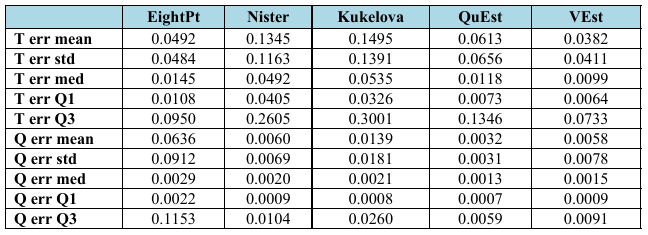
\includegraphics[width=\linewidth]{fig01_QuEstP.png}
      \end{center}
      \caption{QuEst+ module output error statistics on KITTI dataset, running with EightPoint, Nister, Kukelova, QuEst and VEst algorithms for pose estimation.}
    \end{figure}

    \begin{figure}[H]
      \begin{center}
        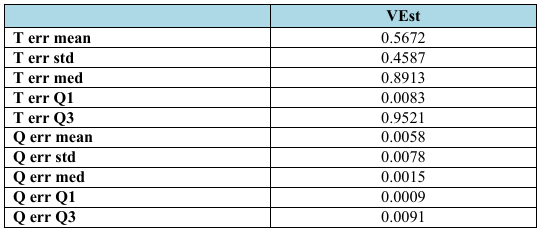
\includegraphics[width=\linewidth]{fig02_VEstP.png}
      \end{center}
      \caption{VEst+ module output error statistics on KITTI dataset, running only with the VEst algorithm for velocity estimation.}
    \end{figure}


    \begin{figure}[H]
      \begin{center}
        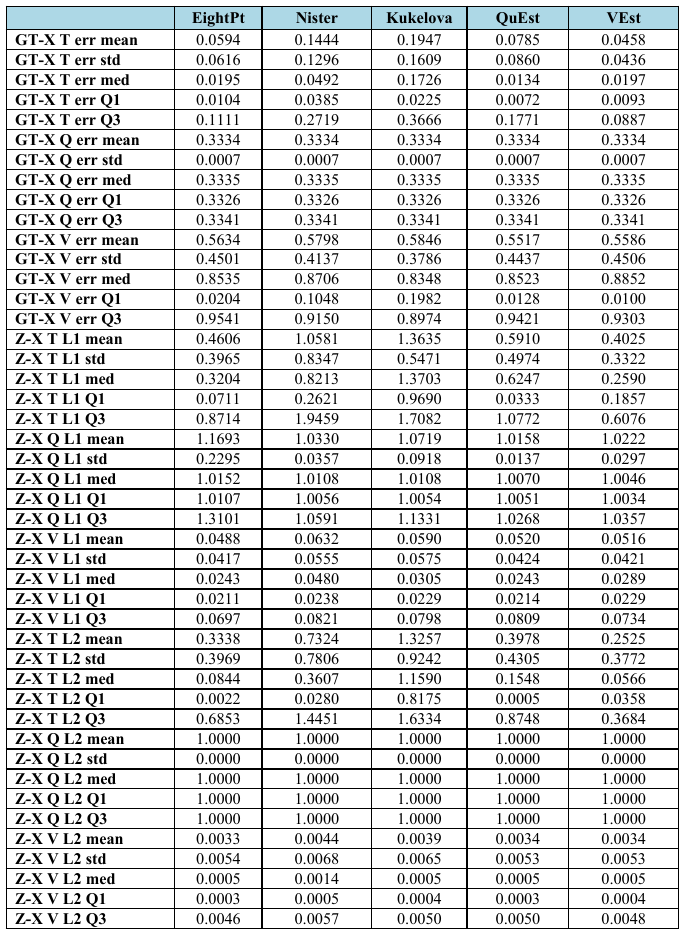
\includegraphics[width=\linewidth]{fig03_QEKF.png}
      \end{center}
      \caption{QEKF module output error statistics on KITTI dataset, running with various pose estimation algorithms.}
    \end{figure}

    \item XEst - Semantic segmentation (\textcolor{red}{RAL - April 30st, 2022}):
    I found \cite{ballester2021dot} for semantic segmentation of moving cars and
    pedestrians. The matched feature points that are labelled as moving object
    will be removed from pose and velocity estimation methods as their inclusion
    results in increased error.

    \item DLO Dataset: There are number of recent papers that have made
    significant contribution to real-time manipulation of DLOs,
    \cite{zhang2021deformable}, \cite{zhang2020robots}, \cite{narang2021sim},
    and \cite{laezza2021reform}. Based on my understanding at the moment, the
    are two main approaches for real-time manipulation of DLO, quasi-static and
    non-quasi-static approaches. Quasi-static modeling of a DLO defines our
    initial approach where we aimed to model the object in form of a set of
    dynamic segments with locally linear dynamic behavior. Non-quasi-static
    approaches define the system as inherently non-linear and aim to model the
    system in a non-linear and often latent space. The two are two completely
    different regimes of mathematical analysis and the manipulation task of DLOs
    the latter is the superior approach. MuJuCo is the only state of the art
    contact-based physics engine that was designed from ground up for this
    specific purpose. In addition, it has built-in API with Unity rendering
    engine which also features API for digital twin, business intelligence and
    ROS. Please see attachments for more detailed analysis. Moreover, for
    dynamic dataset collection, we need a high frequency auto-annotation system
    to capture accurate dynamics, essentially with every other frame as a UV
    ground truth frame. I can design and build a simple embedded switcher circuit
    for automating that. But this has to be after the XEst paper, or after I
    finish the initial draft.

    \item DLO Control: No update.
    \item DLO Perception: No update. -- might not be needed.


    \item Grasping Project (\textcolor{blue}{DLO-03}): I am making this a part of the DLO project.
    \item PyTorch Tutorials: Transfer learning.

  \end{itemize}

\section{Intermediate Goals - Fall 2021:}
\begin{itemize}
      \item QEKF: Finish paper.
      \item UR5e: Do the tutorials.
\end{itemize}

\newpage

%Sets the bibliography style to UNSRT and import the
\newpage
\bibliography{ref}
\bibliographystyle{ieeetr}

\end{document}
